\documentclass[a4paper, 12pt]{article}
\usepackage{apacite}
\usepackage{graphicx}
\usepackage[T1]{fontenc}
\usepackage[utf8]{inputenc}
\usepackage{mathptmx}
\usepackage{enumerate}
\usepackage[margin=0.5in]{geometry}
\usepackage{lipsum}
\usepackage{float}

\renewcommand{\baselinestretch}{1.0}

\newcommand\nd{\textsuperscript{nd}\xspace}
\newcommand\rd{\textsuperscript{rd}\xspace}
\newcommand\nth{\textsuperscript{th}\xspace} %\th is taken already

\setlength\parindent{0pt} % set paragraph indent to zero

% fill up your name, ID and paper title here
\author{
LOA TAT ANN \quad 1221304731 \quad Intro \& Problem Statement, Future Work\\
YU BUI XUAN \quad 241UC24121\quad Methodology, Results\\
MOHAMAD SYAMEL BIN MOHAMAD KARID \quad Discussions, Conclusion\\
% Student Name4 \quad Student ID4 \quad contribution4\\
}
\title{Comparison of Machine Learning Methods Used for Detecting DDoS Attacks in Performance and Accuracy}

\begin{document}
\maketitle

\section{Introduction}
As the world has become increasingly connected, the rapid evolution of network technologies has also led to cyberattacks becoming much more common and harder to contain. This includes DDoS (Distributed Denial of Service) attacks, which try to disrupt network services by overloading a network with malicious traffic (bots) and denying normal system access. \citeA{1} Such attacks can even affect and suffer the largest companies such as the online retailer and cloud service provider Amazon in 2020, where a DDoS attack was detected on its services with a recorded access rate of 2.3 Tbps, and in 2016, where a DDoS attack disrupted a major DNS infrastructure provider which caused several major networks like Twitter (X) and PayPal became inaccessible to users for 3 hours. \citeA{1} 

There are several ways DDoS attacks the host system, including sending malicious traffic at a slow pace to a target (low-rate attacks), using a high amount of packets to compromise the system (high-rate) attacks, exploiting network protocol vulnerabilities to use up resources (protocol exploitation), substituting the IP address of the victim with the attacker's (reflection-amplification). \citeA{1}


To prevent such attacks, various methods are also developed to detect, prevent and mitigate such attacks from harming the system. One such example involves machine learning as they have good performance on network anomaly detection, and it can be adapted to deal with new threats. \citeA{3}

\section{Problem Statement}
Researchers use several different test methods to detect DDoS attacks with machine learning. The main methods are supervised and unsupervised methods. Supervised methods involve a physical network in a lab-based environment where the attacker and the victim exist in the same network and all tests are controlled scientifically. On the flip side, unsupervised methods test the system with real-world networks. The data collected from such methods are analyzed based on their characteristics. A hybrid model uses a combination of the characteristics shown in both methods above. \citeA{1}

\begin{figure}[H]
    \centering
    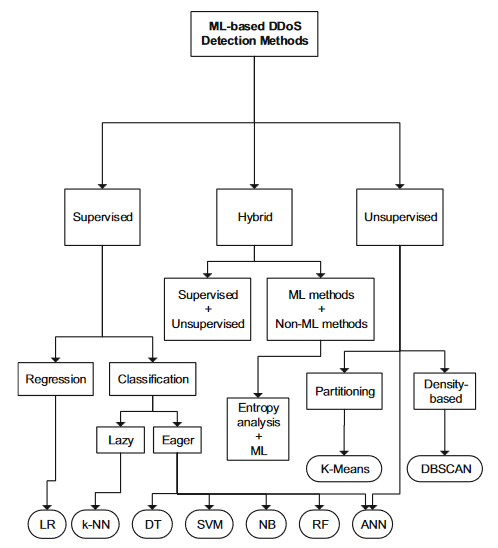
\includegraphics[width=0.7\linewidth]{testt.png}
    \caption{The taxonomy of various ML-based DDoS detection methods \protect\citeA{1}}
    \label{fig:0}
\end{figure}
 
With the development of various methods available, it can be difficult to determine the best method for detecting DDoS networks for a system, as they have different needs and constraints. Furthermore, each detection scenario is different, as they do not always have the same situation and attributes as others. 

This research aims to compare various machine learning models by comparing their accuracy, performance and efficiency of the models regarding detecting DDoS attacks, and determine which methods are suitable for different environments. 

\clearpage

\section{Methodology}
\subsection{TPAAD}
The TPAAD two-phase authentication system, written by Najmun Nisa, Adnan Shahid Khan, Zeeshan Ahmad, and Johari Abdullah, explains a new method that utilizes machine learning algorithms such as Support Vector Machine (SVM) and K-Nearest Neighbors (KNN) to detect DDoS attacks on Software-Defined Networks (SDNs) efficiently. The system also filters incoming packets to detect and stop malicious traffic without host deactivation and affecting normal network connectivity. \citeA{3} The detection for the system, shown in Figure \ref{fig:1} works by utilizing two different modules, which are for detecting threats and mitigating the risks. 

\begin{figure}[H]
    \centering
    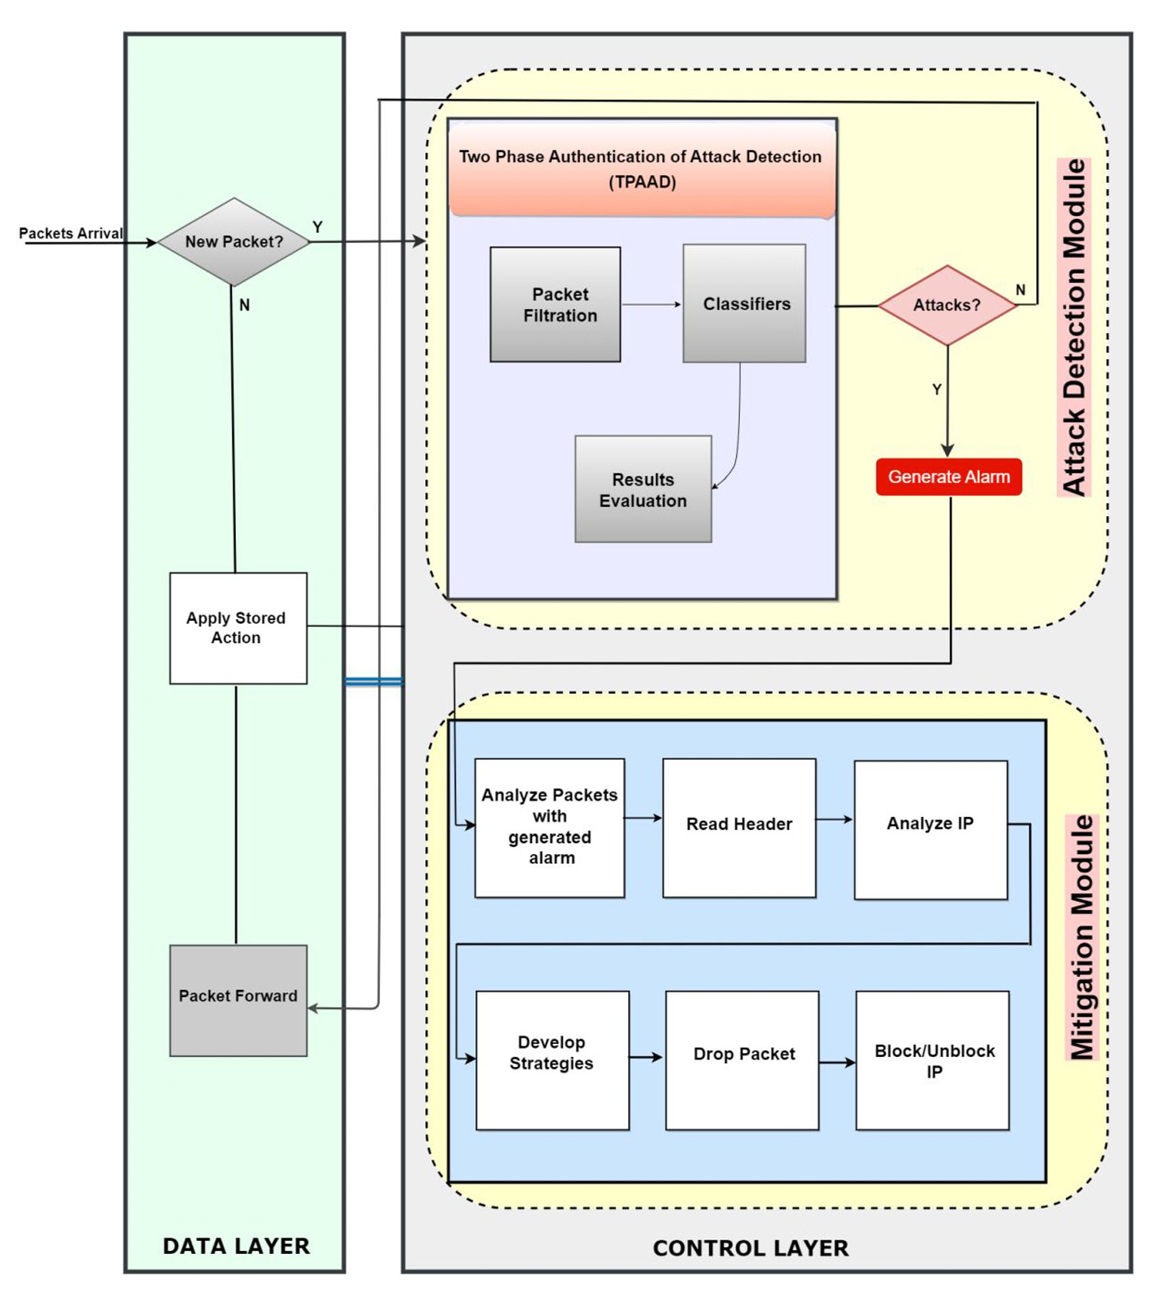
\includegraphics[width=0.7\linewidth]{IMG_0249.jpeg}
    \caption{Diagram for the TPAAD system. \protect\citeA{3}}
    \label{fig:1}
\end{figure}

The detection module continuously monitors the network to identify abnormal traffic. Then packet filtration techniques used by the mitigation module are used to split network traffic to contain and find suspicious activity with machine learning models referring to a predefined dataset (CICDoS 2017). After that, the system employs a tunnelling mechanism to block or reroute malicious traffic ensuring normal network activity is unaffected. \citeA{3}


\subsection{Flexible SDN-Based Architecture}
Low-rate DDoS attacks are more challenging to contain as they target network protocols such as TCP without overloading the system. Because of this, they are harder to detect as they are "integrated" with legitimate network traffic and are difficult to detect and report, and data for such attacks are harder to extract. Hence, the paper proposes a novel modular system architecture to detect such incidents with machine learning techniques. \citeA{4}

Figure \ref{fig:2}, which contains the architecture itself is shown below. The methods used by the system include Support Vector Machines (SVM), Random Forest (RF), K-Nearest Neighbors (KNN), and Multi-Layer Perceptron (MLP).  Important criteria including computing efficiency, false positive rate, and detection accuracy are used to evaluate each method. These models are trained on the CIC DoS 2017 dataset, widely used in DDoS detection research, and the most effective strategy for real-time network protection is determined by analyzing their capacity to distinguish between malicious and legitimate traffic with accuracy. \citeA{4}

\begin{figure}[H]
    \centering
    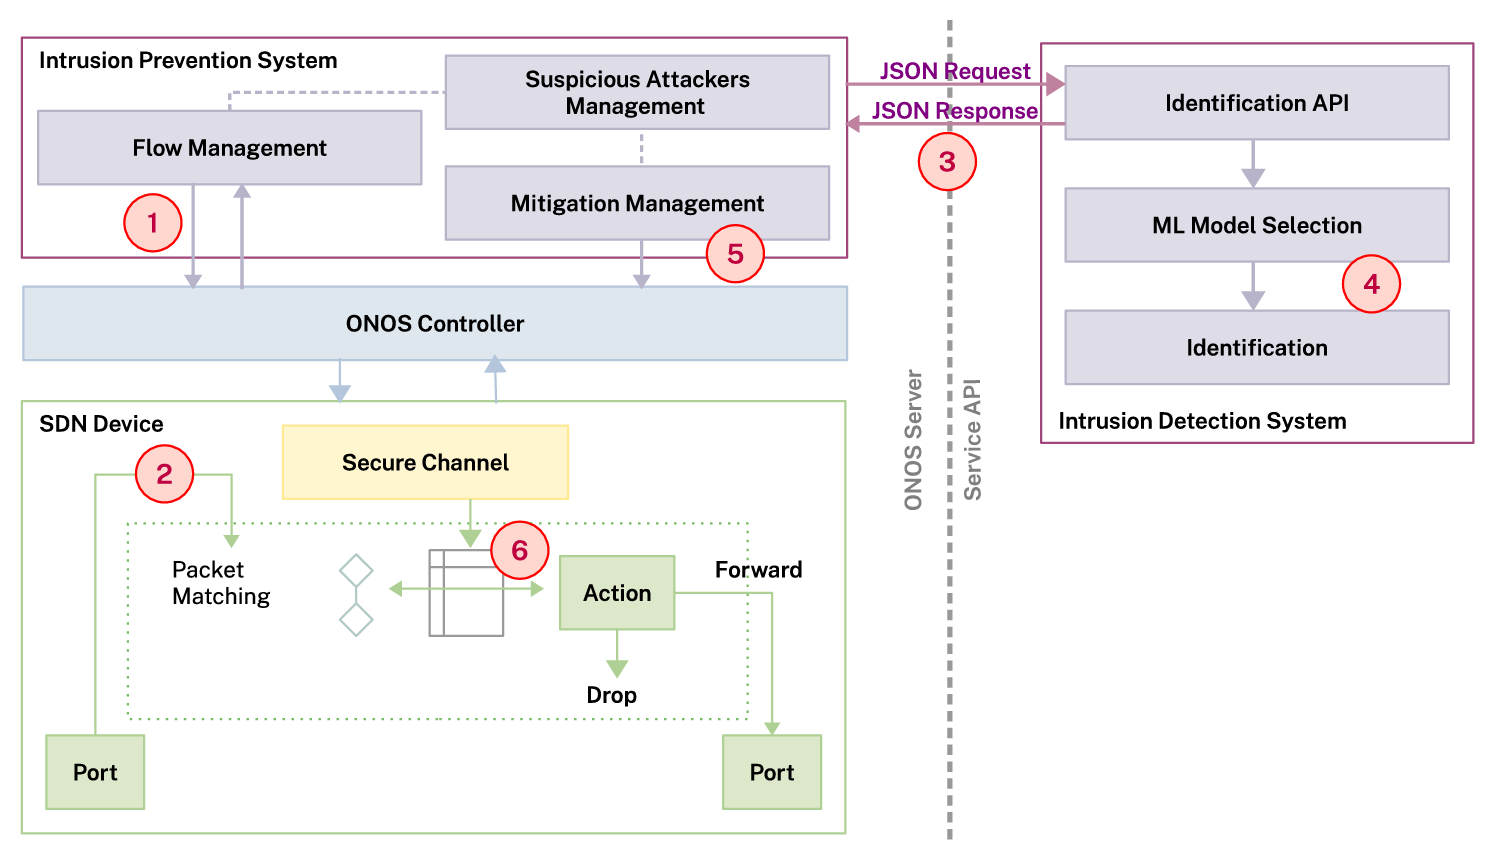
\includegraphics[width=0.7\linewidth]{IMG_0250.jpeg}
    \caption{Diagram for the flexible SDN-based architecture detection system \protect\citeA{4}}
    \label{fig:2}
\end{figure}

\subsection{ML-DDoSnet} 
The methodology in this study focuses on using eight machine learning algorithms to detect and classify Distributed Denial of Service (DDoS) attacks in IoT environments. A variety of models are employed, such as Decision Tree (DT), Random Forest (RF), K-Nearest Neighbors (KNN), Support Vector Machine (SVM), Multilayer Perceptron (MLP), Linear Discriminant Analysis (LDA), and two deep learning approaches: Long Short-Term Memory (LSTM) and Bidirectional LSTM (BiLSTM). The study utilizes the NSL-KDD dataset for training and testing, which includes labelled data (normal or anomalous). Key steps in enhancing model performance by reducing redundant features are feature extraction and selection. Metrics like accuracy, precision, recall, and F1 score are used to compare the models. BiLSTM performs better than the others in terms of identifying DDoS assaults with greater accuracy and reducing false positives. \citeA{5}

\subsection{GRU-LM and Word2vec}
The study proposes a hybrid deep learning method to mitigate DDoS attacks in real-time within mobile networks using Word2vec and a Gated Recurrent Unit Language Model (GRU-LM). The method involves the use of Light Gradient Boosting Machine (LGBM) to detect DDoS attacks with 100\% accuracy. Natural language processing (NLP) techniques are used to enhance the model. Word2vec is used to embed Python source code, and GRU is used to predict the next word in the code sequence. Compared to conventional GRU and LSTM models, this method effectively reduces computational time and memory utilization, which makes it appropriate for real-time DDoS detection in mobile situations. \citeA{6}

The pipeline for the system is shown below in Figure \ref{fig:3}

\begin{figure}[H]
    \centering
    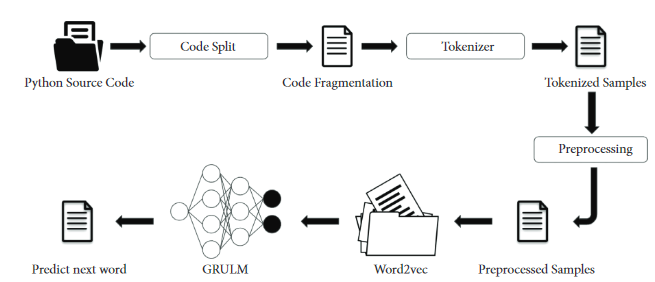
\includegraphics[width=0.7\linewidth]{image-pipe.png}
    \caption{Pipeline used for the experiment. \protect\citeA{6}}
    \label{fig:3}
\end{figure}

\clearpage

\section{Results}

\subsection{TPAAD} 
The tests are used in conjunction with the CICDoS 2017 dataset, and the system is tested with a controlled environment running on an Ubuntu VM on VMWare and an SDN setup created via Mininet and the RYU controller. According to the tests, the TPAAD system recorded a 99.56\% accuracy (higher than the 99.05\% average recorded on other algorithms) with an attack identification false rate of less than 5\% while detecting DDoS attacks. The results are seen in Figure \ref{fig:4} \citeA{3}

\begin{figure}[H]
    \centering
    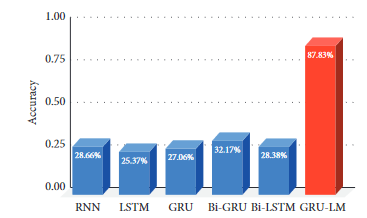
\includegraphics[width=0.7\linewidth]{image.png}
    \caption{Attack detection accuracy comparison of several ML methods \protect\citeA{3}}
    \label{fig:4}
\end{figure}

Besides that, the CPU utilization for the system was recorded at around 9\% when an attack was detected, compared to the 14\% maximum recorded for other algorithms proposed by other researchers. Figures \ref{fig:cpu1} and \ref{fig:cpu2} are the values for the CPU usage recorded before and after a DDoS attack was detected. \cite{3} 

\begin{figure}[H]
    \centering
    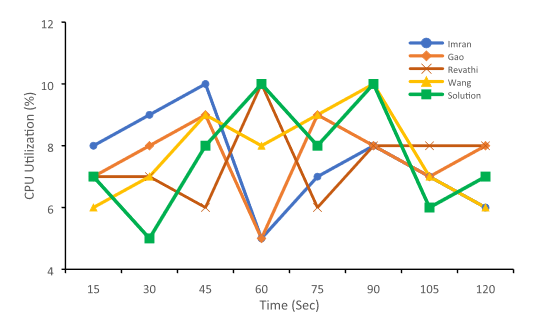
\includegraphics[width=0.7\linewidth]{image-cpu1.png}
    \caption{CPU utilization of different ML methods without DDoS attack. \protect\citeA{3}}
    \label{fig:cpu1}
\end{figure}

\begin{figure}[H]
    \centering
    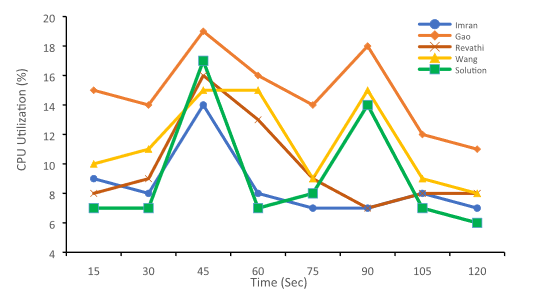
\includegraphics[width=0.7\linewidth]{image-cpu2.png}
    \caption{CPU utilization of different ML methods with DDoS attack. \protect\citeA{3}}
    \label{fig:cpu2}
\end{figure}

\subsection{Flexible SDN-Based Architecture}
In the study, the author established the use of different machine learning models in identifying and preventing Low-Rate DDoS (LR-DDoS) attacks in Software Defined Networks (SDNs). Specifically, as mentioned above, the Multi-Layer Perceptron (MLP) model, which was trained using the CIC DoS 2017 dataset, demonstrated high efficiency in detecting rather complicated kinds of attacks, including Slowloris and GoldenEye. Further, Random Forest and Support Vector Machines (SVM) were also benchmarked and they well performed for the identification of malicious traffic infiltrating the normal traffic. The below models depict how the system adopted the integration of the proposed models through the flexible architecture of the system: The following models show how the system integrated the proposed models for the real-time classification and control of LR-DDoS attacks without affecting legitimate traffic. The capability to alter and modify the machine learning models added to the strength of the architecture and was valuable for protecting SDNs from advanced, periodic low-rate DDoS attacks. \citeA{4}

\begin{figure}[H]
    \centering
    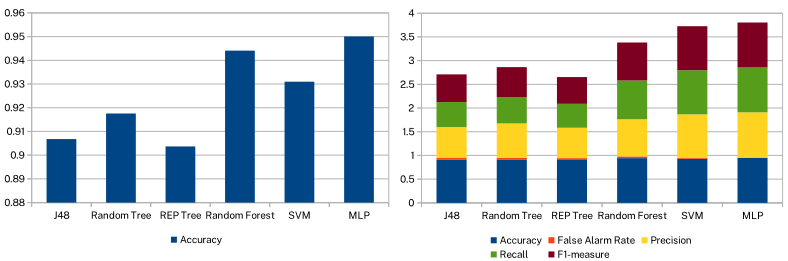
\includegraphics[width=0.8\linewidth]{image_sdn.png}
    \caption{Accuracy estimation and evaluation metric results for the algorithms tested. \protect\citeA{4}}
    \label{fig:sdn}
\end{figure}

\subsection{ML-DDoSnet}

The ML-DDoSnet framework gives a high level of victory in detecting DDoS assaults on IoT networks using machine learning algorithms. The paper used machine learning algorithms including MLP, SVM, RF, and LSTM as well as deep learning algorithms including LSTM, and BiLSTM with an indication that BiLSTM was most effective in the classification of binary and multiclass intrusions. Hence, the NSL-KDD dataset enabled the model to be trained on various attack scenarios, resulting in an effective detection framework. The results showed that BiLSTM achieved higher accuracy and lower false positive rates than other models, and it was more generalizable to unseen attack types. The comparison with the traditional deep learning models showed that the proposed hybrid approach had higher detection rates for real-time IoT DDoS intrusion detection thus presenting a more accurate solution. \citeA{5}

\begin{figure}[H]
    \centering
    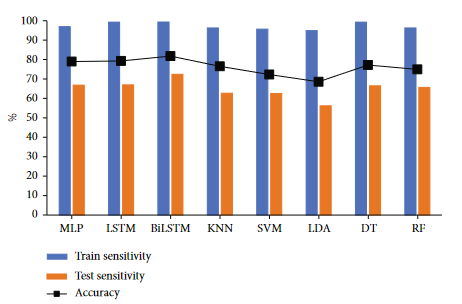
\includegraphics[width=0.7\linewidth]{image-mlddos.png}
    \caption{The accuracy, train sensitivity, and test sensitivity of the proposed approach. \protect\citeA{5}}
    \label{fig:mlddos}
\end{figure}

\subsection{GRU-LM and Word2vec}

The research outcomes reveal that the utilised W2v-GRU\_LM hybrid deep learning forecasted DDoS attacks in mobile circumstances very efficiently and quickly. To prevent and address DDoS attacks, we used the Light Gradient Boosting Machine (LGBM) model to achieve 100\% accuracy, signifying its ability to analyze network traffic intensively. During the second part of the experiment, predicting the next word in Python code achieved an accuracy of 87\%. 3\% improvement on the test set when Word2vec is utilized together with the proposed GRU-Based Language Model (GRU-LM) for code generation. Indeed, this is much higher than the accuracy of approximately 30\% for other types of models including RNN and LSTM. The results show how effectively the GRU-LM model avoids excessive memory consumption and computations time which makes it highly suitable for MN applications that are characterized by resource constraints and the necessity of immediate response. \citeA{6}

\clearpage

\section{Discussions}
\subsection{TPAAD}
\subsubsection{Pros}
The Two-Phase Authentication for Attack Detection (TPAAD) system has advantages that help strengthen the protection of Software Defined Networks (SDN) against DoS attacks. First, the system employs a two-factor authentication technique for effectively detecting and tackling DoS attacks to protect the control plane in SDN. Machine learning algorithms such as SVM and KNN are involved especially for the purpose of effective detection and at the same time keeping false alarm rates low as has been evidenced by tests done on the CICDoS 2017 dataset. Also, the system setup enables hosts to be connected again after they cease producing traffic and assists in maintaining a network without hosting all the hosts. The test results can depict performance by yielding lesser detections and less consumption of CPU resources coupled with increasing packet delivery rate. 
\subsubsection{Cons}
However, like most systems, the TPAAD system has some advantages as well as disadvantages. One of them is the challenge of implementing a two-phase authentication plan. This could require power and time to manage the traffic of the network in an efficient manner. This might lead to a such situation where the attack is detected and responded to in a later time, while impacting the overall network performance. Furthermore, managing the reestablishment of host connections might be problematic when it comes to identifying when a host ceases to produce network activity leading to early connections that might have security risks. In addition, the implementation of machine learning models may need updates and training of the models due to new tactics from the attackers, which may need resources.
\subsubsection{Limitations}
As useful as the TPAAD system is, there are limitations that should be addressed to explore possible use cases for the proposed approach. One of the key limitations of the current work is that the ‘’real-world’’ attack patterns that are not well represented in the dataset that is used to train and test the machine learning algorithms are not comprehensively captured in real-life settings. This may reduce the ability of the system to detect other lesser-known kinds of and frequency of attacks. Furthermore, the systems efficacy depends on the precision of the machine learning models, which can be affected by the caliber and variety of the training data. Another drawback is the effect, on network efficiency caused by the processing needed for identifying and preventing attacks. This could be an issue in places with heavy network traffic flow.

\subsubsection{Contributions of The Research}
The paper presents TPAAD or Two-Phase Authentication for Attack Detection that can help to improve the security of Software-Defined Networks (SDNs) and combat DoS attacks. In this paper, packet filtration together with machine learning classification algorithms particularly support vector machine (SVM) and K-nearest neighbours (KNN) approaches have been used to implement threat detection efficiently in an SDN environment using the CICDoS 2017 dataset. From the results collected, the TPAAD system is able to achieve these objectives; false positives are lowered, CPU usage is limited, and packet delivery ratio is increased, thus, independently verifying DoS attacks and their low overhead. Furthermore, the system also permits dynamic host management by reconnection if a host is disconnected from the particular community owing to the reality it is now generating malicious traffic, though the network functionality must not be impact. Collectively, these contributions provide real insight into making and enhancing security in SDNs and offer a practical and sound approach to the DoS problem without affecting the network performance and functionality. 

\subsection{Flexible SDN-Based Architecture}
\subsubsection{Pros}
The proposed architectural design focuses on being flexible and versatile to enhance its capability, in identifying and mitigating Low Rate DDoS (LR-DDoS) attacks, especially within Software Defined Networks (SDN). This flexibility allows it to adapt to network configurations. It Is well suited for practical use, in real-life scenarios. Using machine learning models, like Random Forests and Support Vector Machines (SVM) along with Multi-Layer Perceptron (MLP) plays a role in creating a reliable detection system that delivers accurate results with minimal false alarms. Moreover, the setup of the architecture enables positioning the Intrusion Detection System (IDS) outside the controller to lessen the burden on the controller and uphold system stability. 
\subsubsection{Cons}
Despite its advantages, there are some limitations to the method. The process depends on entropy thresholds during the detection stage which can be difficult to assess for each flow as it necessitates a thorough statistical analysis. Relying on these thresholds could result in normal traffic being mistakenly categorized as low-rate attacks due to variations in traffic patterns, communication protocols and technologies. Moreover, certain algorithms, like a Simple 3-layer Neural Network and AdaBoostM1 were not successful. They were left out of the assessment suggesting constraints, in choosing or optimizing algorithms.
\subsubsection{Limitations}
The effectiveness of the method becomes questionable when there is one instance of data traffic targeting the network; this limitation restricts its usefulness, in specific situations. The framework's reliance on thresholds based on entropy creates difficulties in categorizing traffic because these thresholds are affected by elements, like the type of traffic and communication protocols. Also worth noting is that the existing setup does not integrate machine learning and deep learning approaches that could improve its ability to counter an array of attacks. The system's ability to scale in network structures and practical operational networks is currently being. There are discussions about implementing a targeted testing approach to enhance scalability. 

\subsubsection{Contributions of The Research}
This paper proposes a low-cost and scalable architecture for the detection and prevention of LR-DDoS in SDN. The architecture that applies six machine learning models which include; J48, Random Tree, REP Tree, Random Forest, Multi-Layer Perceptron (MLP) and Support Vector Machines (SVM) gives a high detection rate of 95\% using the Canadian Institute of Cybersecurity (CIC) DoS dataset. The architecture is implemented in a cloud emulated with Mininet and the ONOS controller to obtain a high similarity with the actual production networks. This flexibility makes it possible to incorporate it into large networks; therefore, such products can be widely used in data centre technologies. In this regard, this work greatly benefits the field of network security by presenting a comprehensive approach toward addressing the issues related to LR-DDoS attacks in the context of SDN. 

\subsection{ML-DDoSnet}
\subsubsection{Pros}
ML-DDoSnet offers advantages in detecting intrusions related to denial of service attacks specifically when it comes to Intrusion Detection Systems (IDS). By integrating machine learning models such as Bidirectional Long Short-Term Memory (BiSLTM), the system's ability to classify network traffic into attacker groups accurately is enhanced for effective intrusion detection. The utilization of the BiSLTM technique is widely acknowledged as a method for evaluating Distributed Denial of Service (DDoS) attacks in Internet of Things (IoT) environments and enables the identification of potential risks associated with such attacks. Furthermore, the architecture of the systems allows for the integration of methods, for handling levels of data transmission enabling it to adapt to the features of IoT devices and networks.
\subsubsection{Cons}
While the method has its benefits and strong points to offer users take note of some drawbacks that come with it as well. One significant concern is the risk of overfitting. This happens when the model is excessively trained using the NSL-KDD dataset resulting in difficulties, especially when applying it to data sets. Additionally, the intricacies of the BiLSTM model make the issue worse by demanding computing resources making them less practical for use, such as when resources are limited. Using the NSL-KDD dataset may not accurately reflect the nature of network traffic behaviours and could impact the model's effectiveness, especially in practical scenarios.

\subsubsection{Limitations}
The ML-DDoSnets limitations point out areas that can be enhanced further along the way because of its low specificity score that may lead to alarms and unnecessary interventions, for network administrators to deal with earnestly while also grappling with the demands of BiLSTM models in IoT setups where resources are typically scarce, especially for real-time processing purposes. The constraints emphasize the importance of improving and testing the model to make it more effective and efficient, in IoT environments so that it can adequately handle the changing network threat environment. 

\subsubsection{Contributions of The Research}
The paper enriches the discussion on IoT security by proposing a new IDS, namely ML-DDoSnet that is tailored to detect DoS attacks in IoT settings. It is a system that applies deep learning approaches including BiLSTM models that enhance the detection of such attacks’ reliability. To accomplish the goal of the study, the improved NSL-KDD dataset is used, which is the refined version of the KDD Cup 99 dataset and free from problems like redundancy and the presence of irrelevant records that are characteristic of older datasets. Furthermore, the work addresses the issues associated with IoT networks, including the heterogeneity of devices and the complicated nature of traffic, by creating a system that addresses these issues, thereby contributing to the IoT security solution that is viable for use in the real world.

\subsection{GRU-LM and Word2vec}
\subsubsection{Pros}
There are benefits to the methods and approaches covered in the research. A noticeable strategy focusing on consistency works well for detecting DDoS attacks. Applications that require real-time responses must be able to achieve accuracy levels while balancing resource usage, which is something that this technique accomplishes. Furthermore, ensemble algorithms like Random Forests, Support Vector Machines, and SWELL demonstrate accuracy in identifying DDoS attacks, proving their dependability in classification tasks. Additionally, accuracy is greatly improved when Conditional Random Field is integrated with CNN for intrusion detection. This demonstrates how feature selection and learning models together can perform well in practical situations.
\subsubsection{Cons}
Even though these methods have some benefits they also have their disadvantages that have to be looked into as well. In the sequence-based model, window size is one of the critical parameters that determine how well the model performs. This may need some changes to work in real time. Ensemble algorithms are generally high performers but they pose a large complexity especially where resources are concerned in the training and execution phases. As we incorporate feature selection with CNN, it increases requirements and the risk of overfitting if not facilitated in the right manner. Although these methods are efficient it is crucial to approach their application with care and have proper management of them implemented.
\subsubsection{Limitations}
The limitations of these methods are obvious in how they were applied and expanded in scope. Generating code using machine learning models like LSTM faces challenges with models like Transformer GPT. This indicates a trade-off between model complexity and performance because of reduced accuracy. While the DeepCom model, used for annotating Java code obtains a decent BLEU score it still falls short of human-level comprehension capabilities which highlights the difficulty of automating code understanding. In addition, character-based generation models with Long Short-Term Memory (LSTM) also face larger computing costs and possible semantic association problems in huge corporations, even though their performance improves with more cells. These limitations underline the need for constant refining and adaption of these strategies to enhance their effectiveness and applicability.

\subsubsection{Contributions of The Research}
This paper proposes a new hybrid deep learning model which is the integration of GRU language model with Word2Vec to improve code generation, especially by exploiting the structural relationship between Python and English languages. It also shows the ability to use and implement machine learning and deep learning in the detection of DDoS attacks and the processed LGBM model with an accuracy of 100\% which is very suitable for real-time network security. In addition, the proposed model yields 87\% of accuracy to predict the next words in the Python source code, which is more accurate as compared to other models in different code prediction tasks and hence the proposed model is efficient and effective. Further, the research identifies the model’s direct and lightweight architecture as a key advantage by offering the best of both time and accuracy, and shows how it can be easily deployed for mobile applications, which is important when dealing with constantly changing and resource-limited environments.

\clearpage

\section{Conclusion}

There are some pros and cons of such methods. For example, The TPAAD system records good accuracy, but it fails with scalability and its reliance of a single controller. \citeA{3} The ML-DDoS system has a high accuracy in IoT environments and is flexible but it suffers in computational cost and scalability. \cite{4} It has proven that all of the systems have their strengths and weaknesses, and from there they have their use case that works perfectly for them. 

Every problem must have a solution, but the best solution depends on the use case and other factors. DDoS attacks are still a major concern for Internet network services, and the challenge remains. Despite this, machine learning will still need more work to have the best results in detecting threats, in a balanced approach that combines cost and performance equally. As the need for cybersecurity and machine learning evolves, the collaboration of all parties involved will be crucial to protecting our networks from such incidents. 

\section{Future work}

We have identified several enhancements for the work done to improve ML in the detection of DDoS systems. The first one is the development of a hybrid system which includes an implementation of various techniques used by previous papers to improve detection speed and adaptability in various scenarios as most of the research in this field focuses only on a handful of methods. Besides that, performance is a major concern of the system, as faster and lighter models provide better speed in detection and could dramatically reduce computational use which can be used on smaller systems with limited resources. We could also use newer and/or more datasets to improve the identification capabilities ensuring even the latest threats could be easily detected. Also, an implementation of such systems in a diverse architecture consisting of different machines and networks ensure the reliability and scalability on even the largest networks. Finally, the system can be developed with different architectures in mind, ensuring all systems can be used with the same system creating a more robust and adaptive framework. 

\clearpage

\bibliographystyle{apacite}
\bibliography{MyBib}{}


\end{document}

